% \section{podstawowe definicje}
% ewentualnie dodać definicje 
% \begin{itemize}
%     \item afinicznej niezależności
% \end{itemize}
W tej części, zdefiniujemy pojęcie wielościanu, oraz inne powiązane z nim definicje i własności.


\section{sympleksy}
\begin{defi}
    Niech punkty $p_0, p_1, \cdots, p_n$ będą afinicznie niezależne w przestrzeni $\mathbb{R}^m$. Wtedy \emph{n-sympleksem} rozpiętym na punktach $p_0, p_1, \cdots , p_n$ (oznaczmy $\Delta(p_0, p_1, \cdots , p_n)$ ) nazwiemy podzbiór punktów $p$ należących do przestrzeni $\mathbb{R}^m$ spełniających
    \[p=\lambda_0 p_0+ \lambda_1 p_1 +\cdots + \lambda_n p_n\]
    \[\sum _{i=0}^n \lambda_i = 1, \;\; \lambda _i\geq 0 \;\forall i=0,1,\ldots,n\]
    Wagi $\lambda_i, i=0,1,\ldots,n$ nazywane \emph{współrzędnymi barycentrycznymi}, są wyznaczone jednoznacznie.
    \begin{figure}[H]
        \centering
        % 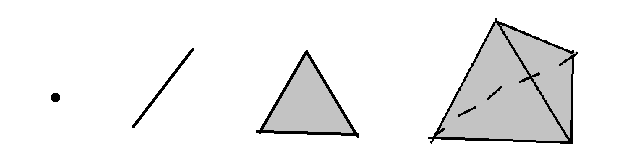
\includegraphics[width=0.8\textwidth]{pictures/sympleksy.png}
        
\begin{tikzpicture}[scale=1.2]

% ============================================
% 1. PUNKT
% ============================================
\begin{scope}[shift={(-4,0)}]
    \fill (0,0) circle[radius=3pt];
\end{scope}

% ============================================
% 2. ODCINEK
% ============================================
\begin{scope}[shift={(-2,0)}]
    \draw[thick] (0,-1) -- (0,1);
    \fill (0,-1) circle[radius=2pt];
    \fill (0,1) circle[radius=2pt];
\end{scope}

% ============================================
% 3. TRÓJKĄT
% ============================================
\begin{scope}[shift={(0,-0.5)}]
     \fill[gray!20] (0,0) -- (2,0) -- (1,1.5) -- cycle;
    \draw[thick] (0,0) -- (2,0) -- (1,1.5) -- cycle;
    \fill (0,0) circle[radius=2pt];
    \fill (2,0) circle[radius=2pt];
    \fill (1,1.5) circle[radius=2pt];
\end{scope}

% ============================================
% 4. OSTROSŁUP TRÓJKĄTNY
% ============================================
\begin{scope}[shift={(4,-0.5)}]
    \tdplotsetmaincoords{70}{120}
    \begin{scope}[tdplot_main_coords, scale=0.8]
        
        % Wierzchołki
        \coordinate (A) at (0,0,0);
        \coordinate (B) at (2,0,0);
        \coordinate (C) at (0.5,1.5,0);
        \coordinate (S) at (0.8,0.6,2.5);
        
        \fill[gray!20] (S) -- (C) -- (B) -- cycle;
        
        % Krawędzie podstawy
        \draw[thick] (B)-- (C);
        \draw[dashed] (B) -- (A);
        \draw[dashed] (C) -- (A);
        
        % Krawędzie boczne
        \draw[thick] (S) -- (C);
        \draw[thick] (S) -- (B);
        \draw[dashed] (S) -- (A);
        
        % Wierzchołki
        \fill (A) circle[radius=2pt];
        \fill (B) circle[radius=2pt];
        \fill (C) circle[radius=2pt];
        \fill (S) circle[radius=2pt];
        
    \end{scope}
\end{scope}

\end{tikzpicture}
        \caption{0,1,2,3-sympleksy w przestrzeni $\mathbb{R}^3$}
        \label{fig:sympleksy}
    \end{figure}
\end{defi}
Inna znana definicja sympleksu to $\Delta(p_0, p_1, \cdots , p_n)=conv(\{p_0, p_1, \cdots , p_n\})$, czyli najmniejszy zbiór wypukły, zawierający punkty $p_0, p_1, \cdots , p_n$. Łatwo możemy pokazać, że będzie to również zbiór zwarty w $\mathbb{R}^m$

Zauważmy, że kożystając z jednoznaczości współrzędnych barycentrycznych, wszystkie $n$-sympleksy będą wzajemnie homeomorficzne, a dodając do tego ciągłość rzutowania na współrzędne, możemy pokazać ich homeomorficzność z hiperkostką $I^n$, z czego od razu dostajemy, że wymiar pokryciowy każdego $n$-sympleksu będzie dokładnie $n$. 

Teraz wprowadzimy kilka pomocniczych definicji

\begin{defi}
    \emph{k-wymiarową ścianą} n-sympleksu rozpiętego na punktach $p_0, p_1, \ldots, p_n$ $(0\le k\le n)$ nazwiemy każdy k-sympleks rozpięty na punktach $p_{i_0}, p_{i_1},\ldots, p_{i_k}$ dla parami różnych $0\le i_j\le n$, $0\le j\le k$.\\
    0-wymiarowe ściany nazwiemy \emph{wierzchołkami}, \\
    \emph{brzegiem}, nazwiemy zbiór $S$ - zbiór wszystkich k-wymiarowych ścian,
    dopełnienie brzegu - \emph{wnętrzem}.
\end{defi}

\section{wielościany}
\begin{defi}
    \emph{Kompleksem symplicjalnym} (lub po prostu kompleksem), nazwiemy dowolną skończoną rodzinę $\mathcal{K}$ sympleksów w przestrzeni euklidesowej spełniającą:
    \begin{itemize}
        \item jeżeli sympleks $S$ należy do $\mathcal{K}$, to każda ściana $S_0$ sympleksu $S$, również należy do $\mathcal{K}$,
        \item jeżeli sympleksy $S_1, S_2$ należą do kompleksu $\mathcal{K}$, to ich przecięcie $S_1 \cap S_2$ jest puste lub jest ścianą obu sympleksów.
    \end{itemize}
    0-sympleksy w $\mathcal{K}$ nazywamy \emph{wierzchołkami}, a każdą podrodzinę $\mathcal{K}_0\subset \mathcal{K}$ która też jest kompleksem nazwiemy \emph{podkompleksem $\mathcal{K}$}.
    \begin{figure}[H]
        \centering
        % 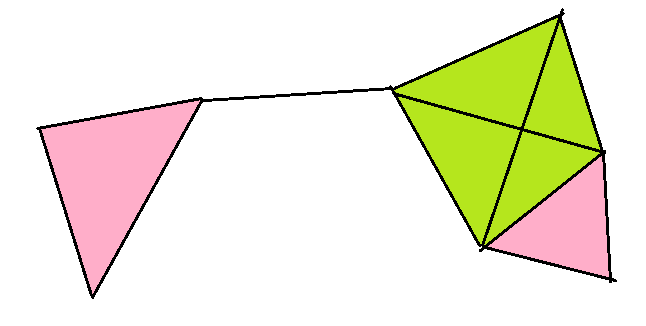
\includegraphics[width=0.8\textwidth]{pictures/kompleks.png}
        \resizebox{0.8\textwidth}{!}{%
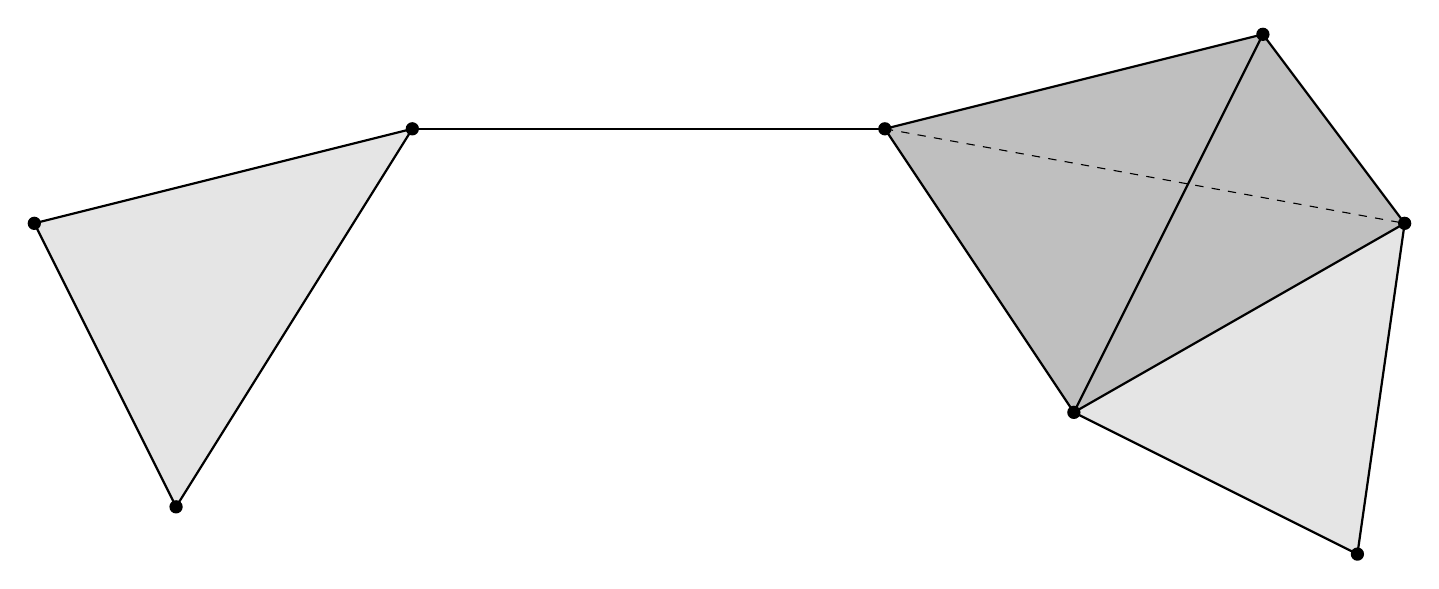
\begin{tikzpicture}[scale=1.2]

\begin{scope}[shift={(0,0)}]
        \coordinate (A) at (-3,0);
        \coordinate (B) at (2,0);
        \coordinate (C) at (-7,-1);
        \coordinate (D) at (-5.5,-4);
        \coordinate (E) at (6,1);
        \coordinate (F) at (4,-3);
        \coordinate (G) at (7.5,-1);
        \coordinate (H) at (7,-4.5);

        \fill[gray!20] (A) -- (C) -- (D) -- cycle;
        \fill[gray!20] (F) -- (G) -- (H) -- cycle;
        \fill[gray!50] (B) -- (E) -- (G) -- (F) -- cycle;
        
        \draw[thick] (A) -- (C) -- (D) -- cycle;
        \draw[thick] (B) -- (A);
        \draw[thick] (B) -- (E) -- (G) -- (F) --cycle;
        \draw[thick] (G) -- (H) -- (F);
        \draw[thick] (E) -- (F);
        \draw[dashed] (B) -- (G);
        
        % Wierzchołki
        \fill (A) circle[radius=2pt];% node[below] {$A$};
        \fill (B) circle[radius=2pt];% node[below] {$B$};
        \fill (C) circle[radius=2pt];% node[below] {$C$};
        \fill (D) circle[radius=2pt];% node[above] {$D$};
        \fill (E) circle[radius=2pt];% node[above] {$E$};
        \fill (F) circle[radius=2pt];% node[above] {$F$};
        \fill (G) circle[radius=2pt];% node[above] {$G$};
        \fill (H) circle[radius=2pt];% node[above] {$H$};
\end{scope}

\end{tikzpicture}
}
        \caption{kompleks symplicjalny}
        \label{fig:kompl}
    \end{figure}
\end{defi}
\begin{przy}
       
% todo przykład
przykład
\end{przy}
% todo wymiar kompleksu
\begin{defi}
    Jeżeli $\mathcal{K}$ jest kompleksem symplicjalnym, to \emph{bryłą} nazwiemy zbiór punktów
    \[|\mathcal{K}|=\bigcup \{S:S\in \mathcal{K}\}\]
\end{defi}

\begin{defi}
    Każdy zbiór $W\in R^n$ dla którego istnieje kompleks symplicjalny $\mathcal{K}$ taki, że $W=|\mathcal{K}|$ 
    nazwiemy \emph{wielościanem}. $\mathcal{K}$ nazwiemy \emph{triangulacją}
\end{defi}
Przez wymiar wielościanu, uznamy wymiar największego $n$-sympleksu zawierającego się w jego triangulacji. Łatwo możemy pokazać, że tak wybrane $n$ nie zależy od wybranej triangulacji, a jedynie od samego wielościanu. Tak zdefiniowaną wartość, nazwiemy wymiarem geometrycznym wielościanu. Wynika zatem, że dla wielościanu wymiar geometryczny i pokryciowy pokrywają się. 

Warto zauważyć, że współrzędne barycentryczne można przedłużyć z sympleksów do całego wielościanu:\\ mając wielościan $K=|\mathcal{K}|$ kompleksu $\mathcal{K}$ oraz jego wierzchołki $p_0, \ldots, p_k$ każdy punkt $p\in K$ możemy reprezentować przez
\[p=\lambda_0 p_0+\cdots +\lambda_k p_k\]
dla $\lambda_0 +\cdots +\lambda_k=1$ oraz $\lambda_i\ge 0\;\;\; \forall i=0, \ldots, k$.
Oczywiście też, jeżeli $\lambda_{i_j}>0$, $j=0, \ldots, l$ to punkt $p$ musi zawierać się w $l-$sympleksie $\Delta(p_{i_0}, \ldots, p_{i_l})$. Jest to również najmniejszy (ze względu na wymiar) sympleks zawierający punkt $p$.\\
Korzystając z tak wprowadzonych współczynników, zdefiniujemy tak zwane \emph{gwiazdy}.

\begin{defi}
    Dla każdego wierzchołka $p_i$ kompleksu symplicjalnego $\mathcal{K}$, \emph{gwiazdą rozpiętą w punkcie $p_i$} nazwiemy zbiór
    \[
     \St_{\mathcal{K}}(p_i) = 
     |\mathcal{K}| \backslash \bigcup\{ S\in \mathcal{K}\;|\;p_i\not \in S\}
    \]
    \begin{figure}[H]
        \centering
        % 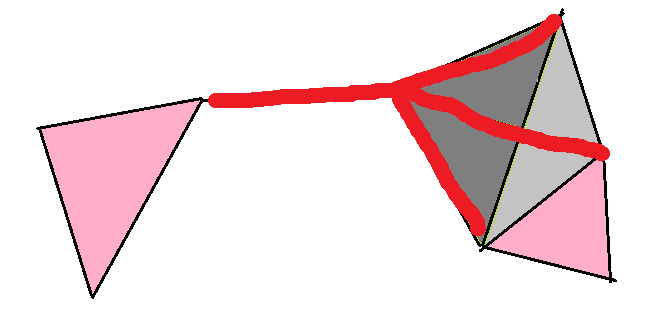
\includegraphics[width=0.8\textwidth]{pictures/gwiazda.png}
        \resizebox{0.8\textwidth}{!}{
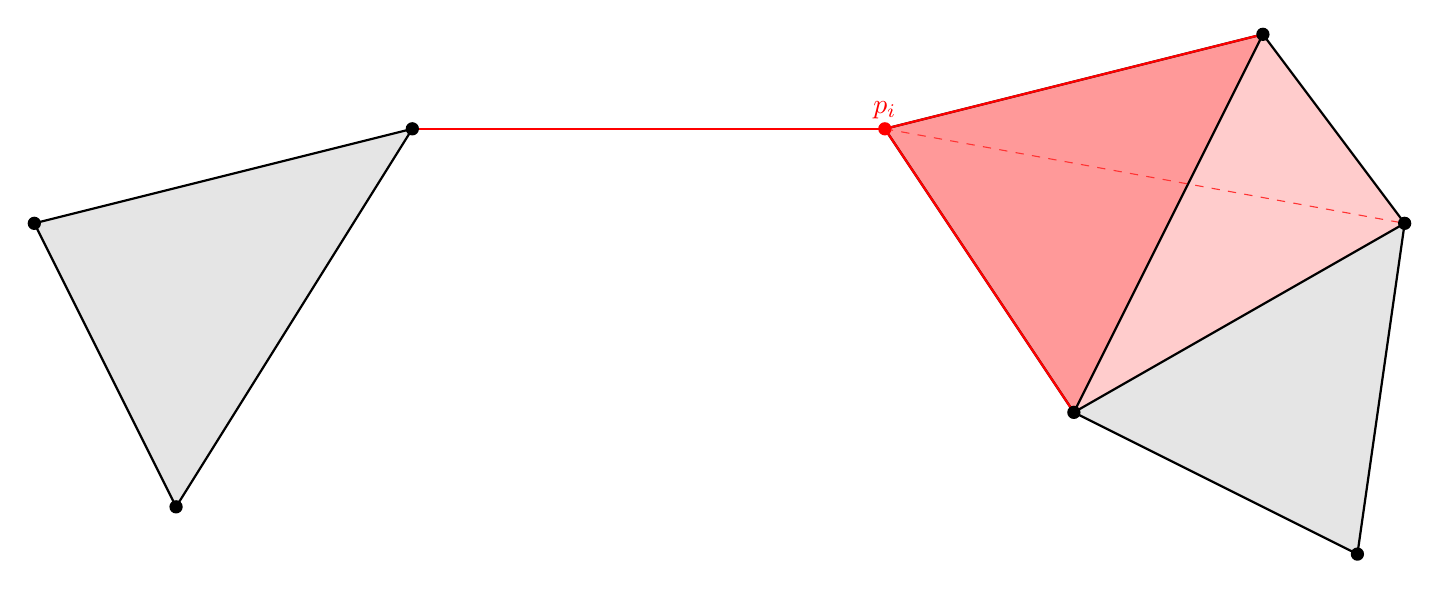
\begin{tikzpicture}[scale=1.2]

\begin{scope}[shift={(0,0)}]
        \coordinate (A) at (-3,0);
        \coordinate (B) at (2,0);
        \coordinate (C) at (-7,-1);
        \coordinate (D) at (-5.5,-4);
        \coordinate (E) at (6,1);
        \coordinate (F) at (4,-3);
        \coordinate (G) at (7.5,-1);
        \coordinate (H) at (7,-4.5);

        \fill[gray!20] (A) -- (C) -- (D) -- cycle;
        \fill[gray!20] (F) -- (G) -- (H) -- cycle;
        \fill[gray!50] (B) -- (E) -- (G) -- (F) -- cycle;

        
        \fill[red!40] (F) -- (E) -- (B) -- cycle;
        \fill[red!20] (F) -- (G) -- (E) -- cycle;
        
        \draw[thick] (A) -- (C) -- (D) -- cycle;
        \draw[red!100][thick] (B) -- (A);
        \draw[thick] (B) -- (E) -- (G) -- (F) --cycle;
        \draw[thick] (G) -- (H) -- (F);
        \draw[thick] (E) -- (F);
        \draw[red!80][dashed] (B) -- (G);
        \draw[red!100][thick] (B) -- (E);
        \draw[red!100][thick] (B) -- (F);
        
        % Wierzchołki
        \fill (A) circle[radius=2pt];% node[below] {$A$};
        \fill[red!100] (B) circle[radius=2pt] node[above] {$p_i$};
        \fill (C) circle[radius=2pt];% node[below] {$C$};
        \fill (D) circle[radius=2pt];% node[above] {$D$};
        \fill (E) circle[radius=2pt];% node[above] {$E$};
        \fill (F) circle[radius=2pt];% node[above] {$F$};
        \fill (G) circle[radius=2pt];% node[above] {$G$};
        \fill (H) circle[radius=2pt];% node[above] {$H$};
\end{scope}

\end{tikzpicture}
}
        \caption{Gwiazda}
        \label{fig:gwiazda}
    \end{figure}
\end{defi}
Łatwo możemy pokazać, że 
$
\St_{\mathcal{K}}(p_i) = 
     \{ p\in |\mathcal{K}|\;:\;\lambda_i>0\}
$,
z czego wynika, że gwiazdy są otwartymi podzbiorami wielościanu $|\mathcal{K}|$

Mimo, że technicznie kompleksy symplicjalne i wielościany są innymi obiektami, w dalszej części pracy będziemy je utożsamiać ze sobą, w części której nam jest to potrzebne używać własności kompleksu symplicjalnego, w innej odpowiadającemu mu wielościanu.
